\documentclass[a4paper,12pt]{article}
\usepackage[utf8]{inputenc}
\usepackage[top=18mm,left=22mm]{geometry}
\textwidth16.9cm\textheight24.8cm
%\usepackage{drafts}\pagestyle{drafts}
\usepackage{amsmath,amssymb,amsthm,amsfonts}
\usepackage{lineno,url}\usepackage{float}
\floatstyle{plaintop}\restylefloat{table}
\usepackage[tableposition=top]{caption}\setlength{\textfloatsep}{6mm} 
\usepackage{graphicx,epsfig}
\usepackage{multirow}\usepackage{pstricks}\usepackage{fancyvrb}
\usepackage{listings,paralist, longtable}
%\usepackage{mathptmx}      % use Times fonts if available on your TeX system
\newcommand{\btab}[2]{\begin{tabular}{#1}#2\end{tabular}}
\def\sm{\small}\def\rb{\raisebox}
\def\twi{\textwidth}\def\ig{\includegraphics}
\def\bmip{\begin{minipage}{\textwidth}}\def\emip{\end{minipage}}
\def\huga#1{\begin{gather} #1 \end{gather}}
\def\hugast#1{\begin{gather*} #1 \end{gather*}}
\def\hual#1{\begin{align} #1 \end{align}}
\def\hualst#1{\begin{align*} #1 \end{align*}}
\def\hueq#1{\begin{equation} #1 \end{equation}}
\def\hueqst#1{\begin{equation*} #1 \end{equation*}}
%%%%%%%%%%%%%%%%%%%%%% Hannes Def %%%%%%%%%%%%%%%%%%%%%%%%%%%%%%
\def\ddt{\frac{{\rm d}}{{\rm d}t}}\def\id{{\rm Id}}
\def\nab{\nabla}\def\eex{\hfill\mbox{$\rfloor$}}
\def\Lam{\Lambda}\def\sign{{\rm sign}}
\newtheorem{theorem}{Theorem}%[section]
\newtheorem{lemma}[theorem]{Lemma}
\newtheorem{remark}[theorem]{Remark}
\newtheorem{example}[theorem]{Example}
\newtheorem{exercise}[theorem]{{}\hs{-1mm}}
\def\bexe{\begin{exercise}}\def\eexe{\eex\end{exercise}}
\def\bsol{\begin{solution}}\def\esol{\eex\end{solution}}
\def\bexa{\begin{example}}\def\eexa{\end{example}}
\def\brem{\begin{remark}}\def\erem{\end{remark}}
\def\bthm{\begin{theorem}}\def\ethm{\end{theorem}}
\def\blem{\begin{lemma}}\def\elem{\end{lemma}}
\def\bcor{\begin{corollary}}\def\ecor{\end{corollary}}
\def\bdefi{\begin{definition}}\def\edefi{\end{definition}}
\newcommand{\R}{{\mathbb R}}
\newcommand{\C}{{\mathbb C}}\newcommand{\N}{{\mathbb N}}
\newcommand{\Q}{{\mathbb Q}}\newcommand{\Z}{{\mathbb Z}}
\newcommand{\Ha}{{\cal H}}
\newcommand{\argmax}{\operatornamewithlimits{argmax}}
\newcommand{\trace}{\operatorname{tr}}
\def\huc#1{{\magenta #1}}\def\pdep{{\tt pde2path}}
\def\bsub{\begin{subequations}}\def\esub{\end{subequations}}
\newcommand{\bmm}{\footnotesize \bpm}\newcommand{\emm}{\epm\normalsize}
\newcommand{\bsmm}{\begin{large}\left(\begin{smallmatrix}}
\newcommand{\esmm}{\end{smallmatrix}\right)\end{large}}

\newfloat{Algorithm}{ht}{lop}[section]

\def\CC{{\cal C}}\def\CK{{\cal K}}\def\CT{{\cal T}}\def\CU{{\cal U}}
\def\CV{{\cal V}}\def\CA{{\cal A}}\def\CE{{\cal E}}\def\CD{{\cal D}}  
\def\CF{{\cal F}}\def\CG{{\cal G}}\def\CH{{\cal H}}\def\CL{{\cal L}}
\def\CO{{\cal O}}\def\CP{{\cal P}}\def\CR{{\cal R}}\def\CS{{\cal S}}
\def\CM{{\cal M}}\def\CN{{\cal N}}\def\CZ{{\cal Z}}\def\CB{{\cal B}}
\def\CX{{\cal X}}\def\CY{{\cal Y}}
\def\OO{{\cal O}}\def\del{\delta}
\def\ga{\gamma}\def\om{\omega}\def\th{\theta}\def\uh{\hat{u}}\def\vh{\hat{v}}
\def\noi{\noindent}\def\ds{\displaystyle}\def\lap{\Delta}\def\al{\alpha}
\def\vt{\vartheta}\def\Id{\mbox{Id}}\def\pa{{\partial}}\def\lam{\lambda}
\def\Ga{\Gamma}\def\Om{\Omega}\def\Del{\Delta}
\def\dd{\, {\rm d}}\def\ri{{\rm i}}\def\sech{{\rm sech}}\def\er{{\rm e}}
\newcommand{\bi}{\begin{itemize}}\newcommand{\ei}{\end{itemize}}
\newcommand{\ben}{\begin{enumerate}}\newcommand{\een}{\end{enumerate}}
\newcommand{\bci}{\begin{compactitem}}\newcommand{\eci}{\end{compactitem}}
\newcommand{\bcen}{\begin{compactenum}}\newcommand{\ecen}{\end{compactenum}}
\newcommand{\bce}{\begin{center}}\newcommand{\ece}{\end{center}}
\newcommand{\reff}[1]{(\ref{#1})}\newcommand{\ul}[1]{{\underline {#1}}}
\newcommand{\mbf}[1]{{\mathbf{#1}}}\newcommand{\ov}[1]{{\overline {#1}}}
\newcommand{\nonu}{\nonumber}\newcommand{\spr}[1]{\left\langle #1 \right\rangle}
\newcommand{\sprb}[1]{\left\langle #1 \right\rangle}
\newcommand{\hs}[1]{{\hspace{#1}}}\newcommand{\vs}[1]{{\vspace{#1}}}
\newcommand{\bhs}[1]{\mbox{\hspace{#1}}}
\def\eps{\varepsilon}\def\epsi{\epsilon}\def\aqui{\Leftrightarrow}
\def\ra{\rightarrow}\def\Ra{\Rightarrow}\def\la{\leftarrow}
\def\lra{\leftrightarrow}\def\lora{\longrightarrow}\def\loma{\longmapsto}
\newcommand{\barr}{\begin{array}}\newcommand{\earr}{\end{array}}
\newcommand{\bpm}{\begin{pmatrix}}\newcommand{\epm}{\end{pmatrix}}
\newcommand{\bsm}{\left(\begin{smallmatrix}}
\newcommand{\esm}{\end{smallmatrix}\right)}
\newcommand{\ba}{\begin{array}}\newcommand{\ea}{\end{array}}

\def\taskip{\renewcommand{\arraystretch}{1}\renewcommand{\baselinestretch}{1}}
\def\teskip{\renewcommand{\arraystretch}{1.05}
\renewcommand{\baselinestretch}{1.025}}
\def\tew{\textwidth}
\def\uold{u_{{\rm old}}}
\def\hulst#1#2{\taskip\lstinputlisting[#1]{#2}\teskip}
\def\pdep{{\tt pde2path}}\def\pdepo{{\tt pde2path}}
\def\PMAXP{Pontryagin's Maximum Principle}
\def\auto{{\tt AUTO}}\def\poc{{\tt p2poc}}
\def\p{\tt p} 
\def\oop{{\tt OOPDE}}\def\pocl{{\tt p2poclib}}
\def\holib{Hopf library}\def\mtom{{\tt mtom}}
\def\mlab{{\tt Matlab}}\def\ptool{{\tt pdetoolbox}}
\def\phome{{\tt www.staff.uni-oldenburg.de/hannes.uecker/pde2path}}
\def\dhome{/hh/path/pde2path/demos/acsuite}
\def\hdhome{/hh/path/pde2path/hopfdemos}
\def\Gbc{G_{\text{BC}}}\def\Qbc{Q_{\text{BC}}}

\definecolor{codegreen}{rgb}{0,0.6,0}
\definecolor{codegray}{rgb}{0.5,0.5,0.5}
\definecolor{codepurple}{rgb}{0.58,0,0.82}
\definecolor{backcolour}{rgb}{0.95,0.95,0.92}
 
\lstdefinestyle{mystyle}{
    backgroundcolor=\color{backcolour},   
%backgroundcolor=\color{white},   
    commentstyle=\color{codegreen},
    keywordstyle=\color{black},
    numberstyle=\small\color{codegray},
    stringstyle=\color{codepurple},
    basicstyle=\footnotesize\ttfamily,
    breakatwhitespace=false,         
    breaklines=true,                 
    captionpos=b,                    
    keepspaces=true,                 
    numbers=left,                    
    numbersep=5pt,                  
    showspaces=false,                
    showstringspaces=false,
    showtabs=false,                  
    tabsize=2, 
stepnumber=1,
language=matlab,  
%firstnumber=1, 
%frame=L,
  xleftmargin=1mm,
}
 
\lstset{style=mystyle}
\def\sss{\subsubsection}\def\fti{\wt f}\def\im{{\rm Im}}
\usepackage{hyperref}
\usepackage{setspace}
\usepackage[inline]{showlabels}\showlabels[\small\color{red}]{cite}\showlabels[\small\color{red}]{ref}\showlabels[\small\color{red}]{bibitem}\renewcommand{\showlabelfont}{\small\ttfamily\color{magenta}}
\def\mpr#1{\cite[#1]{FPBUM24}}

\begin{document}
\noi{\bf Vegetation community patterns},\hfill  \\[2mm]
Michel Ferr\'e$^{1}$, Induja Pavithran$^1$ and Hannes Uecker$^2$,\\
{\footnotesize $^1$ BGU, michel.ferre.diaz@gmail.com and indujap2013@gmail.com, 
$^2$ Institut für Mathematik, Universität Oldenburg
 hannes.uecker@uol.de,
}

\begin{abstract} 
This document presents the {\tt pde2path} implementation of the vegetation community pattern formation problem discussed in reference~\cite{FPBUM24}. The spatial and trait spaces are discretized by a finite element and finite difference approach, respectively. Additionally, we discuss the implementation of the single-species case, where the Busse Balloon is calculated through bifurcation-point continuation. 
\end{abstract}
%\paragraph{General comments.}%\label{imsec}
\def\dhome{../bwhsingle}\def\dname{bwhsingle}
\noi
\tableofcontents

\section{Introduction.}
This tutorial describes the {\tt pde2path} implementation of the community model \cite{FPBUM24}. The community model studies the evolution between different plant species under dryland conditions, where plant species compete for water and light. The community is divided into $N$ functional groups of plant species that differentiate between fast-growing and water stress tolerance species, being quantified by the dimensionless trait space, $0=\chi_0<\chi_1<\dots <\chi_i<\dots<\chi_N=1$, where $\chi_i=i\Delta \chi$ depict the {\it i}th functional group. The spatiotemporal community evolution is described by N continuous fields, $B_i=B_i(\chi_i,x,t)$, with $(i=1,\dots,N)$. The below-ground and above-ground water are modeled by continuous fields $W=W(x,t)$ and $H=H(x,t)$, respectively. Two spatial dependent feedbacks, infiltration and below-ground water diffusion, are considered in their equations. The explicit form of the community model is 
\begin{subequations}\label{eq:Comm}
\begin{eqnarray}
\pa_t B_i&=& \Lambda W B_i - M_i B_i + D_B \partial^2_xB_i + D_\chi \partial^2_\chi B_i,\\
\partial_t W &=& I H - L W - \Gamma W \bar{B} + D_W \partial^2_x W,\\
\partial_t H &=& P - I H + D_H \partial^2_x H,
\end{eqnarray}    
\end{subequations}
where the growth rate of the {\it i}th functional group, $\Lambda_i$, the infiltration rate of above-ground water into soil, $I$, and the evaporation rate, $L$, are written as,
\begin{equation*}
    \Lambda_i \equiv \dfrac{\Lambda_0 K_i}{\bar{B}+K_i}, \quad I\equiv \dfrac{A\left( \bar{\bar{B}}  + f Q\right)}{\bar{\bar{B}}+Q}, \quad L\equiv \dfrac{L_0}{1+R \bar{B}}
\end{equation*}
being $\bar{B}\equiv \sum^N_{i=1}B_i$ and $\bar{\bar{B}}\equiv \sum^N_{i=1}Y_i B_i$; terms that models the interaction the vegetation community and the above/below ground water content. $\partial^2_\chi B \equiv N^2\left( B_{i+1}-2B_i+B_{i-1} \right)$, with $D_\chi$ corresponds to the mutation rate.





\section{Community model: \pdep \, implementation.}
\subsection{Periodic branches.}\label{subsec:PB}
\pdep\, is a MATLAB package that proves a general tool for numerical continuation and bifurcation of nonlinear PDEs combining finite element methods for the spatial discretization with numerical algorithms for continuation and bifurcation methods. The numerical implementation of the system of equations (\ref{eq:Comm}) was based on a finite element approach implemented in \pdep---for detailed background \cite{uecker2021numerical} and a basic introduction see reference \cite{rademacher2018oopde,uecker2019pattern}. The basic setup is made through the files {\tt oosetfemops.m}, file that compute the {\tt FEM} matrices needed, {\tt sG.m} and {\tt sGjac.m}, functions that compute the right-hand side of equations (\ref{eq:Comm}) and its respective (analytical) Jacobian. Additionally, for simplicity, we included a temporal solver based on implicit Euler to find stationary solutions. 

We customize the continuation output display windows through the functions {\tt nplotbra.m} and {\tt cswibra.m}, making use of the functions given by {\tt userplot.m} and their functions related. During continuation additionally, in \pdep, it is possible to calculate on-demand quantifiers such as, in our case, $\chi_{max}$, a quantifier that characterizes the community composition (see reference \cite{FPBUM24}). Table \ref{tb:community} gives an overview of the community model directory.

\taskip
\begin{table}[H]\caption{{\small Scripts and functions in 
{\tt bwhComm}. }}
\bce\vs{-5mm}
{\small 
\begin{tabular}{p{0.14\tew}|p{0.8\tew}}
file&purpose, remarks\\
\hline 
{\tt bwhinit}&initialization of problem struct {\tt p} with standard parameter 
values, call of {\tt stanpdeo1D} to generate a 1D PDE object 
(interval, with mesh),  
initialization of $u$ with $u^*$, call of 
{\tt oosetfemops} to generate the FEM matrices, and finally resetting 
of some \pdep\ parameters to problem-adapted values.\\
{\tt oosetfemops}&assemble and store 
the mass matrix $M$, and the (1-component) Neumann-Laplacian $K$.\\
{\tt nodalf}&``nonlinearity'', i.e., terms without spatial 
derivatives.\\
{\tt sG,sGjac}&rhs of (\ref{eq:Comm}), and Jacobian; these here have a simple standard structure.\\
{\tt sgbra}& output function that provides different functions to be plotted during continuation like $\chi_{max}$. \\
\hline 
{\tt userplot}& function that defines the plotting solution windows during continuation\\
{\tt bbdns}&...\\
\hline
{\tt cmds1}& main script, containing basic \pdep commands, to be run cell-by-cell \\
\end{tabular}
}
\ece
\label{tb:community}
\vs{-5mm}
\end{table}
\teskip

Let us take a look at the \pdep \, implementation. Listing \ref{sG} shows the implementation of the residual. Matrices {\tt p.mat.K} and {\tt p.mat.M} here, which are the stiff and mass matrices, are coded in {\tt oosetfemops.m}, see Listing \ref{ooset}. The {\tt FEM} formulation is then written as,
\begin{eqnarray}
0=-\mathcal{M} F(U) + \mathcal{K}U;
\end{eqnarray}    
where $U:=\left( \tilde{B}_1,\dots,\tilde{B}_N,\tilde{W},\tilde{H} \right)^T\in\mathbb{R}^{n_u}$ the state vector, $\tilde{B}_1=\left(B_{1,1},\dots,B_{1,n_p}\right)$ and $n_u= (N+2) n_p$, being $n_p$ the first discretized plant species and the number of nodes in the {\tt FEM} formulation, respectively. Upper tilde notation $\tilde{(\cdot)}$ depicts the discretized nature of the variable at which it is used. The nonlinear component of our system is written, component-wise, 
\begin{eqnarray*}
    F_i&:=& \Lambda_i \tilde{W} \tilde{B}_i - M_i \tilde{B}_i + D_\chi N^2\left( \tilde{B}_{i+1}-2\tilde{B}_i+\tilde{B}_{i-1} \right),\quad i=(1,\dots,N),\\
    F_{N+1} &:=& \tilde{I}\tilde{H} - L \tilde{W} - \Gamma \tilde{W}\tilde{B},\\
    F_{N+2} &:=& P - \tilde{I}\tilde{H}.
\end{eqnarray*}
To approximate the nonlinear term in the {\tt FEM} formulation we follow \cite{uecker2021numerical}, with $M\in\mathbb{R}^{n_p\times n_p}$ mass matrix given by {\tt p.mat.M}, by $\mathcal{M} F(U)$. The stiff matrix, given by {\tt oosetfemops.m}, approximate the Laplacian operator by $\mathcal{K}U$. The explicit form of $\mathcal{M}$ and $\mathcal{K}$ are given as, 
\begin{equation*}
    \mathcal{M}:= \begin{pmatrix}
        M &\dots & 0 &0 & 0\\
        \vdots& \ddots & 0 & 0& 0 \\
        0&0&M&0&0\\
        0&0&0&M&0\\
        0&0&0&0&M
    \end{pmatrix},\quad \mathcal{K}:= \begin{pmatrix}
        D_B K &\dots & 0 &0 & 0\\
        \vdots& \ddots & 0 & 0& 0 \\
        0&0&D_B K&0&0\\
        0&0&0&D_W K&0\\
        0&0&0&0&D_H K
    \end{pmatrix}
\end{equation*}
where $M\in\mathbb{R}^{n_p\times n_p}$ and $K\in\mathbb{R}^{n_p\times n_p}$. The code for {\tt sG.m} read as,
\lstinputlisting[language=Matlab, caption={{\tt c2Dm/bwhcom/sG.m} provides the calculation of the complete RHS of the system of equations (\ref{eq:Comm}) in finite element formulation. Notice that in line 9, the diffusion coefficients are provided accordingly. },label=sG]{cm2D/bwhcom/sG.m}

The Jacobian is created in the same way, see Listing \ref{sGjac}

\lstinputlisting[language=Matlab, caption={{\tt c2Dm/bwhcom/sGjac.m} computes the Jacobian associated to {\tt sG.m} .},label={sGjac}]{cm2D/bwhcom/sGjac.m}
When coding {\tt sG.m} and {\tt sGjac.m} it is advised to separate the components of the unknow function and the parameters as done here. Except {\tt p.mat.K} and {\tt p.mat.M}, the model is completely implemented now and these two are initialized by {\tt oosetfemops.m}, see Listing \ref{ooset}. 
\lstinputlisting[language=Matlab, caption={{\tt c2Dm/bwhcom/oosetfemops.m} collect the FEM matrices from the PDE object allocated in p.pdeo.  },label={ooset}]{cm2D/bwhcom/oosetfemops.m}
Line 3 introduces the stiffness matrix {\tt K} individually and the mass matrix {\tt M} globally since we need to introduce the diffusion coefficients later in {\tt sGjac.m} file. Notice that we use homogeneous Neumman boundary conditions by only call {\tt assema}. 

Once the community model is fully implemented, to start the continuation, we need to set the \pdep \, environment, model parameters, and initial steady state guess. Listing \ref{bwhinit} gives a basic setting for the present problem. 
\lstinputlisting[language=Matlab, caption={{\tt cm2D/bwhcom/bwhinit.m} collects the minimal initialization commands needed. },label={bwhinit}]{cm2D/bwhcom/bwhinit.m}
Please revise the function {\tt stanparam} (line 2) to obtain a detailed list of initialization commands needed for the use of {\tt pde2path}. Line 4 generates the 1D PDE object by proving the domain length and spacing between mesh points. Line 10, through {\tt p.sw.sfem=-1} assigns the calculation of the FEM matrices by {\tt oossetfemops}, and then calculates them. Lines 11 and 12 set up the bifurcation check method, the use of the explicit Jacobian provided by {\tt sGjac} function and the continuation parameter {\tt par(1)=P}, respectively.

% The main focus is on the interplay of spatial pattern formation 
% and community reassembly under drying trends, i.e., 
% under a decrease of $P$, in the \mlab\ folder {\tt bwhcom}. 
% However, as a preparatory step we also study the single species 
% models with $\chi=0$ and $\chi=1$, respectively, in the folder 
% {\tt bwhsingle}, which we describe first. 

% The community model \reff{m1} is different from the ``standard'' RD system 
% demos of \pdep, and hence requires some special setup. A finite difference approach was performed for convenient and explicit implementation of the continuation files and treatment of the trait space. In this way, the {\tt pde2path} implementation is done by considering $N+2$ partial differential equations, where $N$ corresponds to the functional group $B_i$ plus the two regarded to the above/belowground water $W$ and $H$ equations. See Tab.2 for \mlab\, files, and function description. 

Now we have the basic setting done, we can start the continuation. The file {\tt cmds1.m} give us the basic continuation for the generation of Figure 3 in reference \cite{FPBUM24}.
\lstinputlisting[language=Matlab, caption={{\tt c2Dm/bwhcom/cmds1.m} Basic continuation comands.},label={cmds1}]{cm2D/bwhcom/cmds1.m}
The previous commands produce the following results for the homogeneous solution branch,
\begin{verbatim}
>> cmds1
Problem directory name: comm/hom
creating directory comm/hom
inires=62.2966
res=5.28481e-12, iter=3
step   lambda      y-axis  residual  iter meth   ds       #-EV b(0)       
   0  300.00000    0.65371 5.28e-12    0  nat  0.000e+00   0  1.023e-18 
   1  299.90000    0.65386 5.39e-12    2  nat   -0.10000   0  9.903e-19 
   . . . . . . . . . . . . . . . . . . . . . . . . . . . . . . . . . . 
  21  279.90005    0.68657 6.69e-12    2  nat   -1.00000   0  1.237e-20 
  22  278.90005    0.68837 6.22e-12    2  nat   -1.00000   0  9.656e-21 
   1 possible bifurcation between 278.9 and 277.9, om=0
 checking lam=278.4 ... ok, ineg=2
 checking lam=278.65 ... ok, ineg=0
 checking lam=278.525 ... ok, ineg=1
 checking lam=278.588 ... ok, ineg=1
 checking lam=278.619 ... ok, ineg=0
 mu_r=0.00015167, mu_i=0 
<phi,psi>=-1.6187e-12,BP
  23  2.78619e+02 (BP, saved to comm/hom/bpt1.mat) bisection steps 5, last ds -0.015625
  24  277.90005    0.69019 7.75e-12    2  nat   -1.00000   3  7.514e-21 
  25  276.90005    0.69203 6.54e-12    2  nat   -1.00000   3  5.828e-21 
Timing: total=41.6571, av.step=1.49552, av.Newton=0.829873, av.spcalc=0.182782
Elapsed time is 41.681327 seconds.
\end{verbatim}
Calculating the first Turing mode
\begin{verbatim}
lam=278.6188; 8 smallest eigenvalues: 0.000152   0.00562    0.0181    0.0328    0.0578    0.0644    0.0654    0.0684
using m=3
Problem directory name: comm/T1
step   lambda      y-axis  residual  iter meth   ds       #-EV b(0)       
   stepsizecontrol: dlam=1.27284, res=6.78391e-12, reducing ds to 0.005
   stepsizecontrol: dlam=0.311202, res=3.0601e-09, increasing ds to 0.01
   1 possible bifurcation between 278.619 and 278.93, om=0
 checking lam=278.774 ... ok, ineg=1
 checking lam=278.656 ... ok, ineg=1
 checking lam=278.638 ... ok, ineg=1
 checking lam=278.628 ... ok, ineg=1
 checking lam=278.623 ...nloop: damp alpha=0.5, res=0.000765044
No convergence, localization might be poor ...
 checking lam=278.623 ...nloop: damp alpha=0.5, res=0.000765044
No convergence, localization might be poor ...
 checking lam=278.623 ...nloop: damp alpha=0.5, res=0.000765044
No convergence, localization might be poor ...
mu_r=-0.00119937, mu_i=0, no convergence
   1  278.93000    0.68802 3.06e-09    2  arc    0.00500   1  9.275e-20 
   stepsizecontrol: dlam=0.0099996, res=1.22785e-09, increasing ds to 0.02
   1 possible bifurcation between 278.93 and 278.94, om=0
 checking lam=278.935 ... ok, ineg=2
 checking lam=278.933 ... ok, ineg=2
 checking lam=278.931 ... ok, ineg=2
 checking lam=278.931 ... ok, ineg=2
 checking lam=278.93 ... ok, ineg=2
 checking lam=278.93 ... ok, ineg=2
 checking lam=278.93 ... ok, ineg=2
mu_r=0.0106918, mu_i=0, no convergence
   2  278.94000    0.68799 1.23e-09    1  nat    0.01000   2  2.778e-21 
   stepsizecontrol: dlam=0.0199992, res=1.73947e-08, increasing ds to 0.04
   3  278.96000    0.68794 1.74e-08    1  nat    0.02000   2  1.281e-20 
   stepsizecontrol: dlam=0.0399985, res=5.22826e-12, increasing ds to 0.08
   4  279.00000    0.68783 5.23e-12    2  nat    0.04000   2  1.212e-20 
   stepsizecontrol: dlam=0.0799973, res=1.82201e-11, increasing ds to 0.16
   1 possible bifurcation between 279 and 279.08, om=0
 checking lam=279.04 ... ok, ineg=2
 checking lam=279.06 ... ok, ineg=3
 checking lam=279.05 ... ok, ineg=2
 checking lam=279.055 ... ok, ineg=2
 checking lam=279.057 ... ok, ineg=3
 checking lam=279.056 ... ok, ineg=2
 checking lam=279.057 ... ok, ineg=3
 mu_r=-1.25474e-05, mu_i=0 
<phi,psi>=5.95988e-08,BP
   5  2.79057e+02 (BP, saved to comm/T1/bpt1.mat) bisection steps 7, last ds -0.0003125
   also saved to comm/T1/pt5.mat
   6  279.08000    0.68761 1.82e-11    2  nat    0.08000   3  1.289e-20 
   stepsizecontrol: dlam=0.0799976, res=6.83653e-12, increasing ds to 0.16
   7  279.15999    0.68739 6.84e-12    2  nat    0.08000   3  1.371e-20 
   stepsizecontrol: dlam=0.159996, res=3.29977e-10, increasing ds to 0.32
   8  279.31999    0.68695 3.30e-10    2  nat    0.16000   3  1.547e-20 
   stepsizecontrol: dlam=0.319993, res=9.48978e-09, increasing ds to 0.64
   9  279.63998    0.68607 9.49e-09    2  nat    0.32000   3  1.959e-20 
  10  280.27997    0.68434 6.06e-12    3  nat    0.64000   3  3.039e-20 
  11  280.91996    0.68262 6.80e-09    2  nat    0.64000   3  4.610e-20 
  12  281.55995    0.68091 8.76e-10    2  nat    0.64000   3  6.758e-20 
  . . . . . . . . . . . . . . . . . . . . . . . . . . . . . . . . . . .
 299  383.47742    0.43435 1.06e-11    2  nat    0.64000   0  6.241e-08 
 300  382.83742    0.43430 1.25e-11    2  nat    0.64000   0  6.274e-08 
Timing: total=540.207, av.step=1.71267, av.Newton=0.794449, av.spcalc=0.301111
\end{verbatim}
Calculating the second Turing mode
\begin{verbatim}
Problem directory name: comm/T2
creating directory comm/T2
step   lambda      y-axis  residual  iter meth   ds       #-EV b(0)       

nloopext: damp alpha=0.5, res=19.3513, ds=0.1
   stepsizecontrol: dlam=-3.77511, res=15.383, reducing ds to 0.05

nloopext: damp alpha=0.5, res=55.4696, ds=0.05
   stepsizecontrol: dlam=15.7879, res=1.47795, reducing ds to 0.025
   stepsizecontrol: dlam=10.1701, res=2.13706e-11, reducing ds to 0.0125
   stepsizecontrol: dlam=1.97532, res=1.09421e-11, reducing ds to 0.00625
   stepsizecontrol: dlam=0.388289, res=1.63365e-09, increasing ds to 0.0125
   1 possible bifurcation between 278.619 and 279.007, om=0
 checking lam=278.813 ... ok, ineg=2
 checking lam=278.621 ...nloop: damp alpha=0.5, res=0.00783928
No convergence, localization might be poor ...
 checking lam=278.621 ...nloop: damp alpha=0.5, res=0.00783928
No convergence, localization might be poor ...
 checking lam=278.621 ...nloop: damp alpha=0.5, res=0.00783928
No convergence, localization might be poor ...
 checking lam=278.621 ...nloop: damp alpha=0.5, res=0.00783928
No convergence, localization might be poor ...
 checking lam=278.621 ...nloop: damp alpha=0.5, res=0.00783928
No convergence, localization might be poor ...
 checking lam=278.621 ...nloop: damp alpha=0.5, res=0.00783928
No convergence, localization might be poor ...
mu_r=0.00610572, mu_i=0, no convergence
   1  279.00709    0.68774 1.63e-09    2  arc    0.00625   2  3.450e-19 
   stepsizecontrol: dlam=0.0124997, res=6.78514e-10, increasing ds to 0.025
   1 possible bifurcation between 279.007 and 279.02, om=0
 checking lam=279.013 ... ok, ineg=3
 checking lam=279.01 ... ok, ineg=3
 checking lam=279.009 ... ok, ineg=3
 checking lam=279.008 ... ok, ineg=3
 checking lam=279.007 ... ok, ineg=3
 checking lam=279.007 ... ok, ineg=3
 checking lam=279.007 ... ok, ineg=3
mu_r=-0.0179504, mu_i=0, no convergence
   2  279.01959    0.68771 6.79e-10    1  nat    0.01250   3  5.335e-20 
   stepsizecontrol: dlam=0.0249994, res=9.86429e-09, increasing ds to 0.05
   3  279.04459    0.68764 9.86e-09    1  nat    0.02500   3  8.893e-21 
   stepsizecontrol: dlam=0.0499987, res=6.59872e-12, increasing ds to 0.1
   4  279.09459    0.68751 6.60e-12    2  nat    0.05000   3  1.378e-20 
   stepsizecontrol: dlam=0.0999976, res=7.68363e-12, increasing ds to 0.2
   5  279.19458    0.68725 7.68e-12    2  nat    0.10000   3  1.490e-20 
   stepsizecontrol: dlam=0.199996, res=3.31784e-10, increasing ds to 0.4
   6  279.39458    0.68672 3.32e-10    2  nat    0.20000   3  1.723e-20 
   stepsizecontrol: dlam=0.399993, res=9.9949e-09, increasing ds to 0.8
   7  279.79457    0.68566 9.99e-09    2  nat    0.40000   3  2.284e-20 
   8  280.59456    0.68357 6.06e-12    3  nat    0.80000   3  3.817e-20 
 . . . . . . . . . . . . . . . . . . . . . . . . . . . . . . . . . . . 
 174  413.39413    0.46274 2.26e-09    2  nat    0.80000   3  4.420e-09 
 175  414.19412    0.46081 2.99e-08    2  nat    0.80000   3  5.290e-09 
 176  414.99411    0.45841 1.01e-11    3  nat    0.80000   3  6.712e-09 
nloop: damp alpha=0.5, res=0.0513855
   stepsizecontrol: dlam=0.799971, res=0.0513855, reducing ds to 0.4
   stepsizecontrol: dlam=0.399986, res=2.66083e-11, increasing ds to 0.8
 177  415.39409    0.45671 2.66e-11    3  nat    0.40000   3  7.832e-09 
nloop: damp alpha=0.5, res=0.188948
   stepsizecontrol: dlam=0.799932, res=0.188948, reducing ds to 0.4
nloop: damp alpha=0.5, res=0.0464601
   stepsizecontrol: dlam=0.399966, res=0.0464601, reducing ds to 0.2
   stepsizecontrol: dlam=0.199983, res=1.53913e-08, increasing ds to 0.4
 178  415.59408    0.45528 1.54e-08    3  nat    0.20000   3  8.919e-09 
nloop: damp alpha=0.5, res=0.124661
   stepsizecontrol: dlam=0.399841, res=0.124661, reducing ds to 0.2
nloop: damp alpha=0.5, res=0.0638903
   stepsizecontrol: dlam=0.199921, res=0.0638903, reducing ds to 0.1
nloop: damp alpha=0.5, res=0.0158279
   stepsizecontrol: dlam=0.0999603, res=0.0158279, reducing ds to 0.05
nloop: damp alpha=0.5, res=0.000460114
   stepsizecontrol: dlam=0.0499801, res=0.000460114, reducing ds to 0.025
   stepsizecontrol: dlam=0.0249901, res=3.12767e-08, increasing ds to 0.05
 179  415.61907    0.45495 3.13e-08    2  nat    0.02500   3  9.149e-09 
nloop: damp alpha=0.5, res=0.0140019
   stepsizecontrol: dlam=0.0499587, res=0.0140019, reducing ds to 0.025
nloop: damp alpha=0.5, res=0.000801025
   stepsizecontrol: dlam=0.0249793, res=0.000801025, reducing ds to 0.0125
   stepsizecontrol: dlam=0.0124897, res=9.64975e-10, increasing ds to 0.025
 180  415.63156    0.45472 9.65e-10    3  nat    0.01250   3  9.377e-09 
nloop: damp alpha=0.5, res=0.00441373
   stepsizecontrol: dlam=0.0249585, res=0.00441373, reducing ds to 0.0125
nloop: damp alpha=0.5, res=0.000450962
   stepsizecontrol: dlam=0.0124793, res=0.000450962, reducing ds to 0.00625
   stepsizecontrol: dlam=0.00623964, res=1.74337e-08, increasing ds to 0.0125
 181  415.63779    0.45455 1.74e-08    2  nat    0.00625   3  9.503e-09 
nloop: damp alpha=0.5, res=0.00251158
   stepsizecontrol: dlam=0.0124538, res=0.00251158, reducing ds to 0.00625
nloop: damp alpha=0.5, res=0.000469488
   stepsizecontrol: dlam=0.00622688, res=0.000469488, reducing ds to 0.003125
   stepsizecontrol: dlam=0.00311344, res=3.03109e-08, increasing ds to 0.00625
   1 possible bifurcation between 415.638 and 415.641, om=0
 checking lam=415.639 ... ok, ineg=3
 checking lam=415.64 ... ok, ineg=3
 checking lam=415.641 ... ok, ineg=2
 checking lam=415.64 ... ok, ineg=3
 checking lam=415.64 ... ok, ineg=2
 checking lam=415.64 ... ok, ineg=3
 checking lam=415.64 ... ok, ineg=3
 mu_r=-3.82211e-06, mu_i=0 
<phi,psi>=-2.32234e-07,BP
 182  4.15640e+02 (BP, saved to comm/T2/bpt1.mat) bisection steps 7, last ds 1.2207e-05
 183  415.64091    0.45441 3.03e-08    2  nat    0.00313   2  9.619e-09 
nloop: damp alpha=0.5, res=0.000423671
   stepsizecontrol: dlam=0.00309418, res=0.000423671, reducing ds to 0.0015625
   stepsizecontrol: dlam=0.00154709, res=8.7473e-10, increasing ds to 0.003125
   1 possible bifurcation between 415.641 and 415.642, om=0
 checking lam=415.642 ... ok, ineg=2
 checking lam=415.642 ... ok, ineg=2
 checking lam=415.642 ... ok, ineg=2
 checking lam=415.642 ... ok, ineg=2
 checking lam=415.642 ... ok, ineg=2
 checking lam=415.642 ... ok, ineg=2
 checking lam=415.642 ... ok, ineg=1
 mu_r=1.25927e-06, mu_i=0 
<phi,psi>=-1.8246e-10,BP
 184  4.15642e+02 (BP, saved to comm/T2/bpt2.mat) bisection steps 7, last ds -6.10352e-06
 185  415.64246    0.45429 8.75e-10    3  nat    0.00156   1  9.739e-09 
nloop: damp alpha=0.5, res=0.000403631
   stepsizecontrol: dlam=0.00146613, res=0.000403631, reducing ds to 0.00078125
nloop: damp alpha=0.5, res=0.000163929
   stepsizecontrol: dlam=0.000733066, res=0.000163929, reducing ds to 0.000390625
nloop: damp alpha=0.5, res=4.09644e-05
   stepsizecontrol: dlam=0.000366533, res=4.09644e-05, reducing ds to 0.000195313
   stepsizecontrol: dlam=0.000183267, res=4.83095e-09, increasing ds to 0.000390625
 186  415.64264    0.45426 4.83e-09    2  nat    0.00020   1  9.765e-09 
nloop: damp alpha=0.5, res=0.000105241
   stepsizecontrol: dlam=0.000325408, res=0.000105241, reducing ds to 0.000195313
nloop: damp alpha=0.5, res=2.63406e-05
   stepsizecontrol: dlam=0.000162704, res=2.63406e-05, reducing ds to 9.76563e-05
   stepsizecontrol: dlam=8.13519e-05, res=5.56829e-08, increasing ds to 0.000195313
 187  415.64272    0.45421 5.57e-08    4  nat    0.00010   1  9.801e-09 
   stepsizecontrol: dlam=-0.000272382, res=1.42743e-08, increasing ds to 0.000390625
   1 possible bifurcation between 415.643 and 415.642, om=0
 checking lam=415.643 ... ok, ineg=0
 checking lam=415.643 ... ok, ineg=0
 checking lam=415.643 ... ok, ineg=0
 checking lam=415.643 ... ok, ineg=0
 checking lam=415.643 ... ok, ineg=0
 checking lam=415.643 ... ok, ineg=0
 checking lam=415.643 ... ok, ineg=0
 mu_r=0.000163737, mu_i=0 
<phi,psi>=-0.0444386, Fold
 188  415.64245    0.45414 1.43e-08    1  arc    0.00020   0  9.919e-09 
   stepsizecontrol: dlam=-0.000183715, res=4.36202e-11, increasing ds to 0.000390625
 189  415.64226    0.45411 4.36e-11    2  nat    0.00020   0  9.891e-09 
   stepsizecontrol: dlam=-0.000376292, res=2.66905e-10, increasing ds to 0.00078125
 190  415.64189    0.45408 2.67e-10    2  nat    0.00039   0  9.913e-09 
   stepsizecontrol: dlam=-0.000765194, res=9.64048e-10, increasing ds to 0.0015625
 191  415.64112    0.45403 9.64e-10    2  nat    0.00078   0  9.952e-09 
   stepsizecontrol: dlam=-0.00154559, res=2.54436e-09, increasing ds to 0.003125
 192  415.63958    0.45395 2.54e-09    2  nat    0.00156   0  1.001e-08 
   stepsizecontrol: dlam=-0.00310778, res=5.73319e-09, increasing ds to 0.00625
 193  415.63647    0.45385 5.73e-09    2  nat    0.00313   0  1.009e-08 
   stepsizecontrol: dlam=-0.00623277, res=1.20292e-08, increasing ds to 0.0125
 194  415.63024    0.45370 1.20e-08    2  nat    0.00625   0  1.021e-08 
   stepsizecontrol: dlam=-0.0124829, res=2.45026e-08, increasing ds to 0.025
 195  415.61775    0.45349 2.45e-08    2  nat    0.01250   0  1.039e-08 
   stepsizecontrol: dlam=-0.0249832, res=4.93441e-08, increasing ds to 0.05
 196  415.59277    0.45320 4.93e-08    2  nat    0.02500   0  1.063e-08 
   stepsizecontrol: dlam=-0.0499837, res=9.89227e-08, increasing ds to 0.1
 197  415.54279    0.45280 9.89e-08    2  nat    0.05000   0  1.098e-08 
   stepsizecontrol: dlam=-0.0999843, res=1.08713e-11, increasing ds to 0.2
 198  415.44280    0.45225 1.09e-11    3  nat    0.10000   0  1.179e-08 
   stepsizecontrol: dlam=-0.199985, res=9.9476e-12, increasing ds to 0.4
 199  415.24282    0.45150 9.95e-12    3  nat    0.20000   0  1.263e-08 
   stepsizecontrol: dlam=-0.399987, res=8.04334e-12, increasing ds to 0.8
 200  414.84283    0.45052 8.04e-12    3  nat    0.40000   0  1.384e-08 
 201  414.04284    0.44926 1.15e-11    3  nat    0.80000   0  1.555e-08 
 . . . . . . . . . . . . . . . . . . . . . . . . . . . . . . . . . . . 
 300  334.84276    0.43776 9.88e-12    2  nat    0.80000   0  4.402e-08 
Timing: total=613.351, av.step=1.9546, av.Newton=0.854463, av.spcalc=0.430008
\end{verbatim}
The final lines of the file {\tt cmds1.m} produces the results given in figure (\ref{fig:min_bif})
\begin{figure}
    \centering
    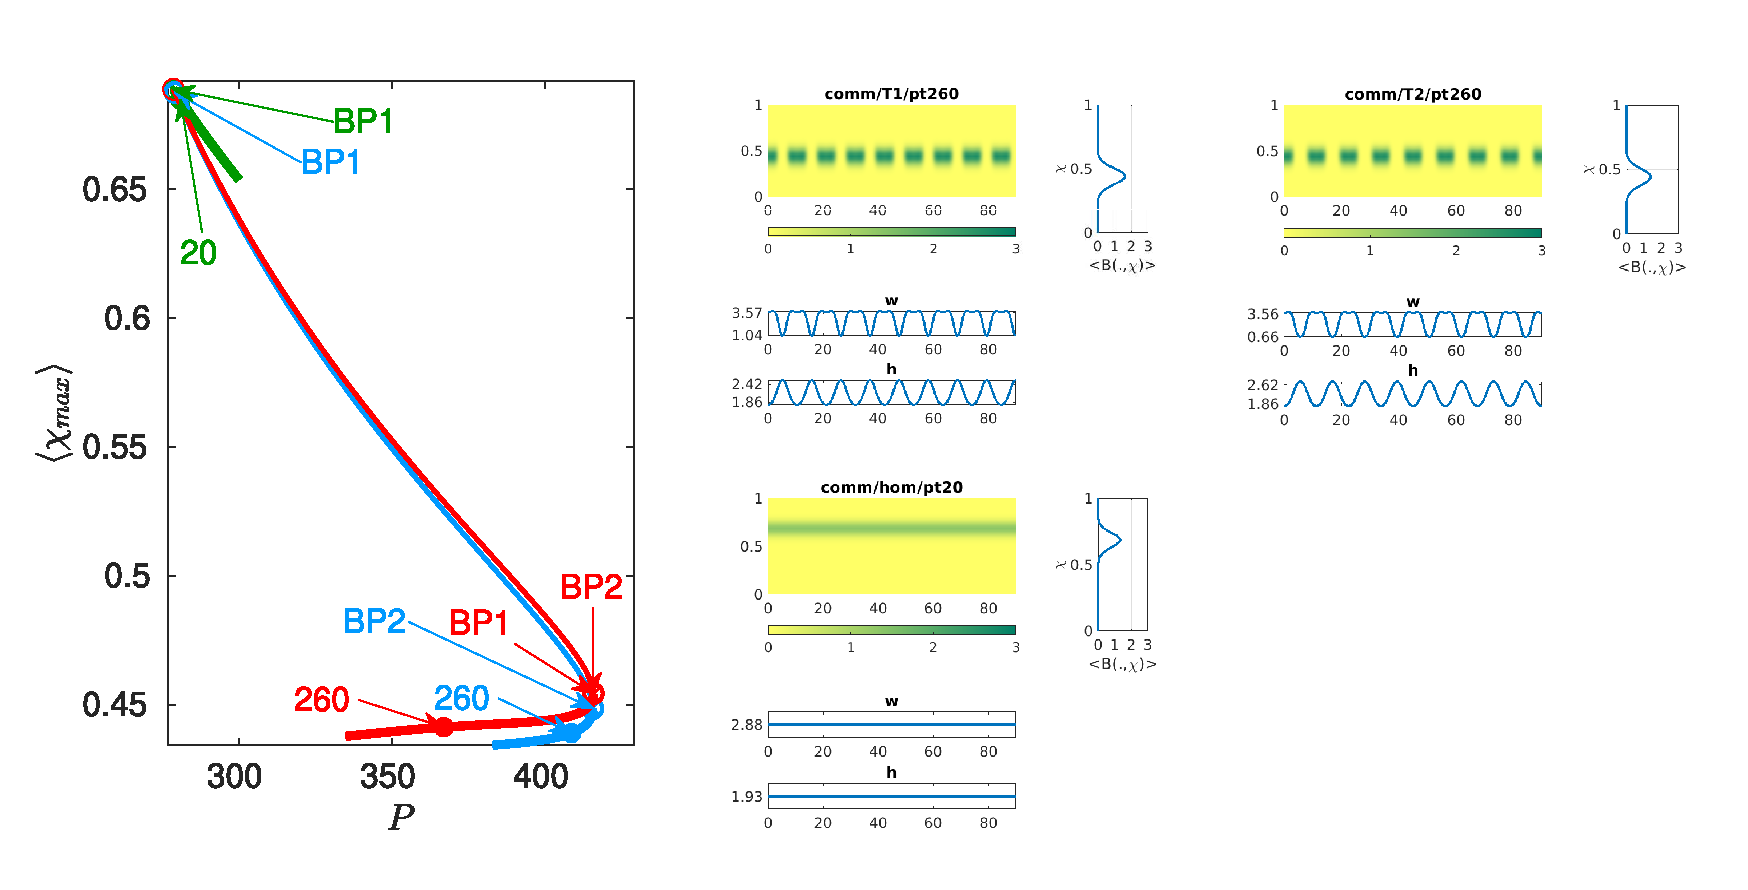
\includegraphics[width=1\linewidth]{min_bif.eps}
    \caption{A minimal bifurcation diagram depicting three states by their respective numbers. Bifurcation points are labeled by {\tt BP}.}
    \label{fig:min_bif}
\end{figure}

\subsection{Brute Force Busse-Balloon.}
In reference \cite{FPBUM24}, we discuss the plant community evolution under precipitation variation, showing the community composition shifts to stress-tolerance species as precipitation decreases for homogeneous solutions, while patterns, due to the increase of water availability, shift back to fast-growing species exhibiting {\it patch thinning} along the periodic branch as precipitation further decreases. Such dynamic is plotted in Figure 3 in reference \cite{FPBUM24}. Additionally, to compare the plant community pattern solutions to the single plant species pattern solutions---for $\chi=1$ and $\chi=0$---we characterize the Busse-Balloon for each and present them in Figure (4) en reference \cite{FPBUM24}. Usually, Busse-Balloon calculation can be done by bifurcation point continuation (see next section \ref{sec:BBs}), which requires extending the discretized system size up to double. This limits us from working on the current community model due to the technical issue (computer resource-wise); consequently, we went for a brute force approach, i.e., calculating the periodic branches, saving the stable ranges, and interpolating the boundaries to generate a smoother result. 
The brute-force Bussee-Balloon code is given as follows,
\lstinputlisting[language=Matlab, caption={{\tt c2Dm/bwhcom/bfbb.m}.}]{cm2D/bwhcom/bfbb.m}
By considering the original data of reference \ref{FPBUM24}, the following file,
\lstinputlisting[language=Matlab, caption={{\tt c2Dm/bwhcom/cmds2.m}.}]{cm2D/bwhcom/cmds2.m}
produces a brute fore Bussee-Balloon (see Figure (\ref{fig:brut_for_bb})).
\begin{figure}
    \centering
    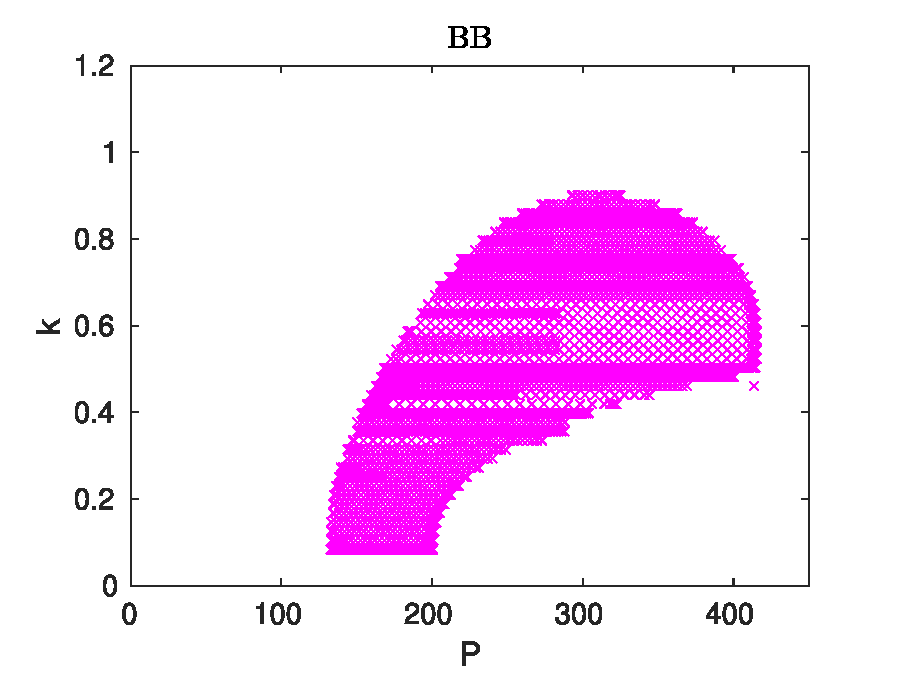
\includegraphics[width=0.6\linewidth]{BBcom.eps}
    \caption{Brute Force Bussee-Balloon using the original data of reference [FPBUM24].}
    \label{fig:brut_for_bb}
\end{figure}


\section{Single species model.}
\subsection{Periodic branches.}
The single species 
models (SSM) 
\begin{subequations}\label{eq:SSM}
\begin{eqnarray}
    \partial_t B_i &=& \Lambda_i W B_i - M_i B_i + D_B \partial^2_x B_i,\\
    \partial_t W &=& I H - L W - \Gamma W \bar{B} + D_W \partial^2_x W,\\
    \partial_t H &=& P - I H + D_H \partial^2_x H 
\end{eqnarray}    
\end{subequations}
is a standard semilinear reaction-diffusion system and hence can be treated similarly to the models in \cite[Ch.9]{uecker2021numerical}, and associated demos 
available at \cite{p2phome}. We also refer to 
\cite{uecker2021numerical,uecker2019pattern} and the tutorials at \cite{p2phome} for general 
background and usage of \pdep. The {\tt bwhsingle} folder comes with the files needed to calculate a minimal version of the bifurcation diagram exhibited in Figure 1 in reference \cite{FPBUM24} and the ones necessary for the Busse Ballon calculation via branch point continuation (BPC). Similar treatment as the \pdep \, implementation treatment gived in section (\ref{subsec:PB}) is given. A list of the pertinent files is given in Table \ref{tab1}. 

\taskip
\begin{table}[H]\caption{{\small Scripts and functions in 
{\tt \dname}. Associated to most {\tt cmds*}--scripts are 
{\tt cmds*plot} scripts for plotting;  
all figure numbers refer to \cite{FPBUM24}. 1st two blocks: scripts; 
3rd block: problem describing functions and overloads of 
\pdep\ library functions and convenience functions. \label{tab1}}}
\bce\vs{-5mm}
{\small 
\begin{tabular}{p{0.14\tew}|p{0.8\tew}}
file&purpose, remarks\\
\hline
{\tt cmds1}&starting script ... Fig.4 \\
\hline 
{\tt bwhinit}&initialization of problem struct {\tt p} with standard parameter 
values, call of {\tt stanpdeo1D} to generate a 1D PDE object 
(interval, with mesh),  
initialization of $u$ with $u^*$, call of 
{\tt oosetfemops} to generate the FEM matrices, and finally resetting 
of some \pdep\ parameters to problem-adapted values.\\
{\tt oosetfemops}&assemble and store 
the mass matrix $M$, and the (1-component) Neumann-Laplacian $K$.\\
{\tt nodalf}&``nonlinearity'', i.e., terms without spatial 
derivatives, called in {\tt hotintxs}.\\
{\tt sG,sGjac}&rhs of (\ref{eq:SSM}), and Jacobian; these here have a simple standard structure.\\
% {\tt nodaljac}&Jacobian of ``nonlinearity'', called in {\tt sGjac}.\\
{\tt bpjac}&
implements $\pa_u(G^T_u\psi)$ for BPC, see \cite[\S3.6.1]{uecker2021numerical}.\\
{\tt sgbra}&mod of library function {\tt stanbra}; \\
% {\tt secobraHPC}&mod of {\tt secobra} used for output during HPC.\\
\hline 
\end{tabular}
}
\ece

\vs{-5mm}
\end{table}
\teskip

\def\dhome{../bwhcom}\def\dname{bwhcom}
% For a deeper discussion about the implementation and theoretical background, please refer to \cite{uecker2021numerical}.

The script files are presented in detail as follows. {\tt bwhinit.m} set up the continuation environment. Please revise the function {\tt stanparam} (line 2) to obtain a detailed list of initialization commands needed for the use of {\tt pde2path}. Line 4 generates the 1D PDE object by proving the domain length and spacing between mesh points, while we assign the calculation of the FEM matrices for {\tt oossetfemops} through {\tt p.sw.sfem=-1} in Line 10, and then calculates them. Lines 11 and 12 set up the bifurcation check method, the use of the explicit Jacobian provided by {\tt sGjac} function ({\tt p.sw.jac=1}) and the continuation parameter {\tt par(1)=P} by {\tt p.sw.bifchek=2}.

\lstinputlisting[language=Matlab, caption={{\tt cm2D/bwhsingle/bwhinit.m} Minimal initialization commands. }]{cm2D/bwhsingle/bwhinit.m}

In {\tt oosetfemops.m}the {\tt FEM} matrices from the PDE object allocated in {\tt p.pde} are obtained and assigned to the {\tt p.mat.K} for the stiffness matrix and {\tt p.mat.M} for the mass matrix. Notice that only the mass matrix is allocated from {\tt oosetfemops.m} since we need to introduce the diffusion coefficient later in {\tt sGjac.m}.

\lstinputlisting[language=Matlab, caption={{\tt cm2D/bwhsingle/oosetfemops.m} collect the FEM matrices.}]{cm2D/bwhsingle/oosetfemops.m}

As in the previous section (\ref{subsec:PB}), we implement the nonlinear terms through the {\tt nodalf.m} file, where the $\chi$-dependent terms are calculated accordingly\footnote{We implement the {\tt FEM} similarly as the subsection (\ref{subsec:PB})}. In line 6, the diffusion coefficients are provided accordingly. 
\lstinputlisting[language=Matlab, caption={{\tt c2Dm/bwhsingle/sG.m} }]{cm2D/bwhsingle/sG.m}
Notice we can make the continuation based on a numerical jacobian; however, for numerical performance, we decided to provide the jacobian explicitly through {\tt p.sw.jac=1}, being the Jacobian calculated by {\tt sGjac.m},
\lstinputlisting[language=Matlab, caption={{\tt c2Dm/bwhsingle/sGjac.m} }]{cm2D/bwhsingle/sGjac.m}

Now we have all set up to continuate some solutions branches by running {\tt cmds1.m},
\lstinputlisting[language=Matlab, caption={{\tt c2Dm/bwhsingle/cmds1.m} }]{cm2D/bwhsingle/cmds1.m}
he previous commands produce the following results,

\begin{verbatim}
    >> cmds1
Problem directory name: s1/hom
step   lambda      y-axis  residual  iter meth   ds       #-EV b(0)       
   0  300.00000    5.23399 7.35e-09    2  nat  0.000e+00   0   49.65399 
   1  299.90000    5.23124 8.80e-12    2  nat   -0.10000   0   49.62790 
. . . . . . . . . . . . . . . . . . . . . . . . . . . . . . . . . . . . 
  59  270.89969    4.34205 6.44e-12    2  nat   -0.50000   0   41.19233 
  60  270.39968    4.32456 7.37e-12    2  nat   -0.50000   0   41.02642 
   1 possible bifurcation between 270.4 and 269.9, om=0
 mu_r=-8.52986e-07, mu_i=0 
<phi,psi>=6.71159e-10,BP
  61  2.70372e+02 (BP, saved to s1/hom/bpt1.mat) bisection steps 10, last ds 0.000244141
  62  269.89968    4.30697 7.80e-12    2  nat   -0.50000   3   40.85954 
. . . . . . . . . . . . . . . . . . . . . . . . . . . . . . . . . . . . 
  79  260.89966    3.96985 7.42e-12    2  nat   -1.00000   3   37.66128 
  80  259.89966    3.92952 8.41e-12    2  nat   -1.00000   3   37.27868 
Timing: total=5.30086, av.step=0.0302019, av.Newton=0.00210061, av.spcalc=0.00616449
\end{verbatim}
First Turing branch
\begin{verbatim}
    lam=270.3719; smallest eigenvalues: -8.53e-07    0.0161    0.0251
using m=3
Problem directory name: s1/T1
creating directory s1/T1
step   lambda      y-axis  residual  iter meth   ds       #-EV b(0)       
   1 possible bifurcation between 270.372 and 271.193, om=0
 mu_r=3.70903e-05, mu_i=0 
<phi,psi>=-3.14952e-10,BP
   1  2.70495e+02 (BP, saved to s1/T1/bpt1.mat) bisection steps 10, last ds 2.44141e-05
   2  271.19298    4.34117 7.47e-12    3  arc    0.05000   3   41.25940 
   3  271.24295    4.34223 8.68e-12    2  nat    0.05000   3   41.27410 
   4  271.34291    4.34436 7.08e-12    2  nat    0.10000   3   41.30347 
   1 possible bifurcation between 271.343 and 271.543, om=0
 mu_r=-2.80281e-05, mu_i=0 
<phi,psi>=-3.26133e-12,BP
   5  2.71347e+02 (BP, saved to s1/T1/bpt2.mat) bisection steps 10, last ds -9.76563e-05
   also saved to s1/T1/pt5.mat
   6  271.54284    4.34862 6.09e-11    2  nat    0.20000   4   41.36214 
   7  271.74277    4.35288 1.86e-11    2  nat    0.20000   4   41.42072 
   1 possible bifurcation between 271.743 and 272.143, om=0
 mu_r=5.64688e-05, mu_i=0 
<phi,psi>=1.48108e-07,BP
   8  2.71887e+02 (BP, saved to s1/T1/bpt3.mat) bisection steps 10, last ds 0.000195313
   9  272.14267    4.36136 1.20e-09    2  nat    0.40000   5   41.53761 
. . . . . . . . . . . . . . . . . . . . . . . . . . . . . . . . . . . . 
 106  341.34391    5.46895 1.10e-11    3  nat    0.02500   5   58.73031 
   1 possible bifurcation between 341.344 and 341.294, om=0
 mu_r=1.05115e-05, mu_i=0 
<phi,psi>=4.9079e-10,BP
 107  3.41316e+02 (BP, saved to s1/T1/bpt4.mat) bisection steps 10, last ds -2.44141e-05
 108  341.29403    5.46407 1.13e-11    3  nat    0.05000   0   58.73642 
 . . . . . . . . . . . . . . . . . . . . . . . . . . . . . . . . . . . . 
 150  310.14468    4.58636 1.20e-11    2  nat    0.80000   0   53.91918 
Timing: total=8.83578, av.step=0.0318982, av.Newton=0.00333239, av.spcalc=0.00495385
\end{verbatim}
Second Turing branch
\begin{verbatim}
    Problem directory name: s1/T2
creating directory s1/T2
step   lambda      y-axis  residual  iter meth   ds       #-EV b(0)       
   1 possible bifurcation between 270.372 and 270.903, om=0
mu_r=-0.0123881, mu_i=0, no convergence
   1  270.90260    4.33107 1.10e-09    2  arc    0.05000   3   41.16361 
   1 possible bifurcation between 270.903 and 270.953, om=0
mu_r=0.0280418, mu_i=0, no convergence
   2  270.95257    4.33207 7.47e-12    2  nat    0.05000   4   41.17817 
   3  271.05252    4.33406 7.59e-12    2  nat    0.10000   4   41.20726 
   4  271.25243    4.33805 1.19e-10    2  nat    0.20000   4   41.26538 
   1 possible bifurcation between 271.252 and 271.652, om=0
 mu_r=-6.60466e-05, mu_i=0 
<phi,psi>=4.38396e-07,BP
   5  2.71272e+02 (BP, saved to s1/T2/bpt1.mat) bisection steps 10, last ds -0.000195313
   also saved to s1/T2/pt5.mat
   6  271.65228    4.34602 5.34e-09    2  nat    0.40000   5   41.38138 
. . . . . . . . . . . . . . . . . . . . . . . . . . . . . . . . . . . . 
 110  338.57778    5.34937 1.33e-11    3  nat    0.10000   5   58.10432 
   1 possible bifurcation between 338.578 and 338.378, om=0
 mu_r=-5.69923e-06, mu_i=0 
<phi,psi>=-1.26009e-08,BP
 111  3.38525e+02 (BP, saved to s1/T2/bpt2.mat) bisection steps 10, last ds 9.76563e-05
 112  338.37789    5.33730 1.11e-11    3  nat    0.20000   0   58.09821 
. . . . . . . . . . . . . . . . . . . . . . . . . . . . . . . . . . . . 
 149  309.77825    4.53834 1.08e-11    2  nat    0.80000   0   53.60794 
 150  308.97824    4.51805 1.08e-11    2  nat    0.80000   0   53.46958 
Timing: total=9.31093, av.step=0.0361994, av.Newton=0.00311805, av.spcalc=0.00558257
\end{verbatim}
We plot the results in Figure (\ref{fig:min_bif_ss}).
\begin{figure}
    \centering
    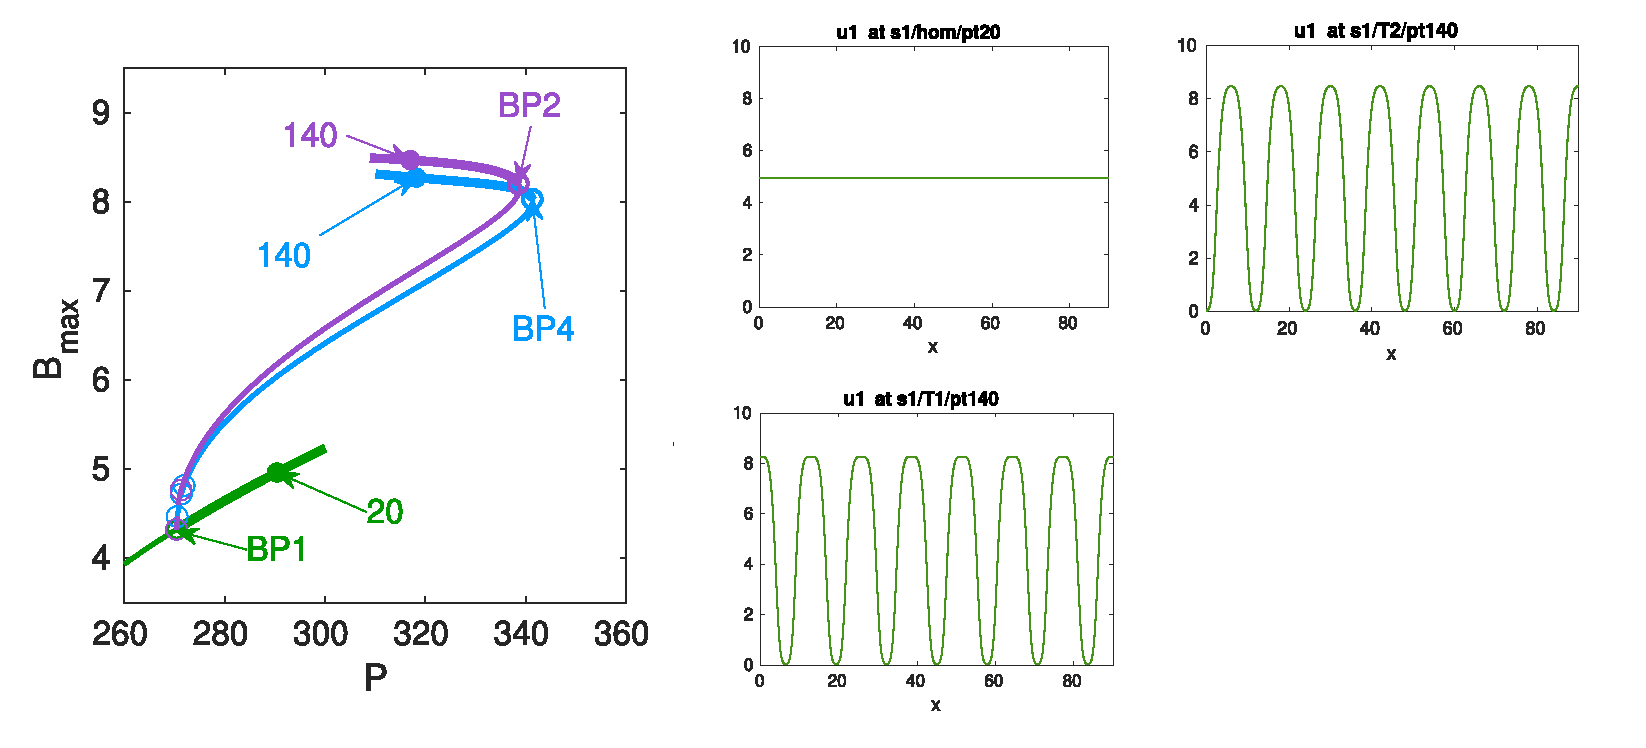
\includegraphics[width=1\linewidth]{min_bif_ss.eps}
    \caption{A minimal bifurcation diagram depicting three states by their respective numbers. Bifurcation points are labeled by {\tt BP}.}
    \label{fig:min_bif_ss}
\end{figure}



\subsection{Busse-Balloon: Bifurcation point continuation.}\label{sec:BBs}

Important special points of solutions branches of (\ref{eq:SSM}) are such fold points (FPs), branch points (BPs), and Hopf points (HPs), and a useful feature of a numerical continuation and bifurcation package is the option of FP-, BP-, and HP-continuation, fow which one hast to free an additional parameter. Besides being important themselves due to topological changes occurring there (and new branches bifurcating at BPs and HPs), FPs, BPs of HPs for instance also often delimit stability regions of solutions branches, and hence FPC, BPC and HPC can be used to efficiently compute such stability regions in dependence of a second parameter. For detailed explanation and background, see references \cite{uecker2021numerical,uecker2023continuation}

The numerical continuation of the bifurcation points 
\begin{align}
    H(U) = \begin{pmatrix}
        G(u,\lambda) + \mu M_d \psi\\
        G^T_u(u,w)\Psi\\
        \parallel\psi\parallel_2^2 - 1\\
        \langle \psi,G_\lambda(u,w)\rangle 
    \end{pmatrix} = \begin{pmatrix}
        0\\0\\0\\0
    \end{pmatrix},\quad U =(u,\psi,w),
\end{align}
where $(u,\lambda)$ is a simple BP (for the continuation in $\lambda$), $\psi$ is an adjoint kernel vector, and $w=(\lambda,\mu)$ with $w_1=\lambda$ the primary active parameter and $w_2 = \mu$ as additional active parameter.

The main task then is to set up $\partial_u (G_u^T \psi)$ for the Jacobian of $H$, e.i.,
\begin{align}
    J_H = \begin{pmatrix}
        G_u & \mu \mathcal{M} & G_\lambda & \mathcal{M}\psi\\
        \partial_u(G_u^T\psi) & G^T_u & \partial_{\lambda(}G_u^T\psi) &0\\
        0 & 2 \psi^T & 0 & 0\\
        \psi^T \partial_\lambda G_u^T & G_\lambda^T & \psi^T \partial_\lambda G_\lambda &0
    \end{pmatrix}
\end{align}
As (\ref{eq:SSM}) is a semilinear problem, we can proceed similarly to the examples given in \cite{p2phome} by implementing $\partial_u (G_u^T \psi)$ explicitly
\begin{align}
    \partial_u (G_u^T \psi) &= \partial_u\begin{pmatrix}
        f_{1,u_1}\psi_1+f_{2,u_1}\psi_2\\
        f_{2,u_1}\psi_1+f_{2,u_2}\psi_2
    \end{pmatrix}\mathcal{M}^T\\
    &=\begin{pmatrix}
        f_{1,u_1u_1}\psi_1 + f_{2,u_1u_1}\psi_2 & f_{1,u_1u_2}\psi_1 + f_{2,u_1u_2}\psi_2\\
        f_{1,u_1u_2}\psi_1 + f_{2,u_2u_1}\psi_2 & f_{1,u_2u_2}\psi_1 + f_{2,u_2u_2}\psi_2
    \end{pmatrix}\mathcal{M}^T
\end{align}

% \lstinputlisting[language=Matlab, caption={{\tt cm2D/bwhsingle/nodalf.m}. This script provides the nodal values of the RHS of (\ref{eq:SSM}), e.i., the terms that do not exhibit spatial derivatives. }]{cm2D/bwhsingle/nodalf.m}

% \lstinputlisting[language=Matlab, caption={{\tt c2Dm/bwhsingle/sGjac.m} computes the Jacobian associated to {\tt sG.m} .}]{cm2D/bwhsingle/sGjac.m}
through {\tt bpjac.m}, given explicitly as follows.
\lstinputlisting[language=Matlab, caption={{\tt c2Dm/bwhsingle/bpjac.m}. This function provides the component $\partial_u\left( G_u\phi\right)$ used for bifurcation-point continuation.  }]{cm2D/bwhsingle/bpjac.m}
Once $\partial_u (G_u^T \psi)$ is implemented, we use the following minimal commands to produce the first step in the Busse-Balloon calculation
\lstinputlisting[language=Matlab, caption={{\tt c2Dm/bwhsingle/cmds2.m} }]{cm2D/bwhsingle/cmds2.m}
Producing the following results for the first continuation ({\tt p.sol.ds>0})
\begin{verbatim}
Warning: Computation may be slow as some pde derivatives are computed numerically.
Approx. zero eigenvalue=1.05115e-05.
New active parameters and their values:
aux vars of p (is point of type 1)
p.nc.ilam  values
  19     1 
  1     341.316 
  20     1.05115e-05 
Problem directory name: bps1a
creating directory bps1a
BP continuation. Use p=bpcontexit(p) to return to normal continuation.
step   lambda      y-axis  residual  iter meth   ds       b(0)       
   0    1.00000  341.31572 3.87e-09    1  nat  0.000e+00   58.73440 
   1    1.00030  341.30625 1.15e-09    2  nat    0.00030   58.73226 
. . . . . . . . . . . . . . . . . . . . . . . . . . . . . . . . . .
  19    1.60194  269.85979 3.47e-09    5  arc    0.02400   41.66268 
  20    1.60778  265.87779 8.62e-10    4  arc    0.02400   40.66906 
Timing: total=16.0294, av.step=0.747914, av.Newton=0.730686, av.spcalc=0
\end{verbatim}
Results for the reverse direction ({\tt p.sol.ds<0}) we obtain,
\begin{verbatim}
Problem directory name: bps1b
creating directory bps1b
BP continuation. Use p=bpcontexit(p) to return to normal continuation.
step   lambda      y-axis  residual  iter meth   ds       b(0)       
   0    1.00000  341.31572 3.87e-09    0  nat  0.000e+00   58.73440 
   1    0.99910  341.34404 3.05e-09    2  nat   -0.00090   58.74081 
. . . . . . . . . . . . . . . . . . . . . . . . . . . . . . . . . . 
  19    0.70554  344.21361 5.88e-12    5  nat   -0.01800   59.49595 
  20    0.70553  344.21359 5.80e-09   10  arc   -0.00001   59.49595 
Timing: total=33.7603, av.step=1.64145, av.Newton=1.62148, av.spcalc=0
\end{verbatim}
Producing the following plot (see Figure (\ref{fig:busse_ball_ss}))
\begin{figure}
    \centering
    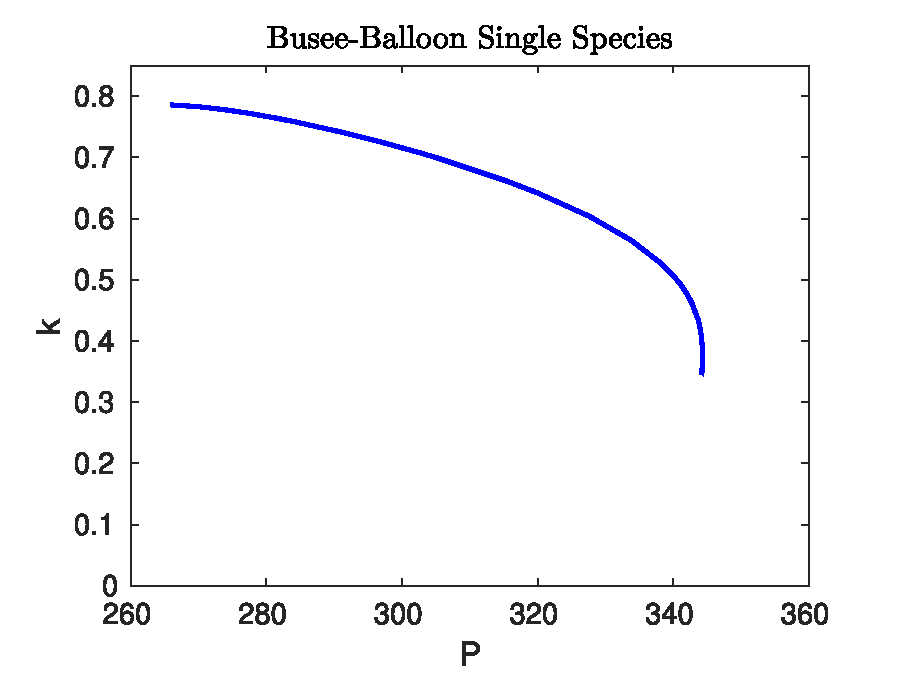
\includegraphics[width=0.6\linewidth]{bussee_balloon.eps}
    \caption{Few of bifurcation point continuation results from {\tt BP4} at the folder {\tt s1/T1}.}
    \label{fig:busse_ball_ss}
\end{figure}



\\
\\
\\



\renewcommand{\baselinestretch}{0.9}
{\small  \bibliographystyle{alpha} 
%\bibliographystyle{plain} 
\bibliography{references}   % name your BibTeX data base
}

\end{document}
